\section{Maxwell Equations}

\subsection{Integral form}
\begin{multicols}{2}
	\textbf{Gauss's law, 1835\newline}
	\noindent The electric flux density $\vec{D} = \varepsilon \vec{E}$ through a closed oriented area $(A)$ is equal to the total electric charge $Q$ which is surrounded by this area.
	\begin{equation}
		\oiint\limits_{\left(\partial\Omega\right)} \vec{D}\left(\vec{r}\right)\cdot d\vec{S}\left(\vec{r}\right) = Q = \iiint\limits_{\left(\Omega\right)}\rho\left(\vec{r}\right)\cdot dV\left(\vec{r}\right)
		\label{eq:MaxwellInt1}
	\end{equation}
	
	\textbf{Coulomb's law, 1785\newline}
	\noindent The magnetic flux trough a closed oriented area is alway zero! This means there are no magnetic monopols.
	\begin{equation}
		\oiint\limits_{\left(\partial\Omega\right)} \vec{B}\left(\vec{r}\right)\cdot d\vec{S}\left(\vec{r}\right) = 0
		\label{eq:MaxwellInt2}
	\end{equation}
	
	\textbf{Ampère's law, 1826\newline}
	The sum of all currents through a closed oriented area can be computed as
	\begin{equation}
		\oint\limits_{\left(\partial S\right)} \vec{H}\left(\vec{r}\right)\cdot d\vec{l}\left(\vec{r}\right) = \sum_{k=1}^{N} I_k = \Theta =  \iint\limits_{\left(S\right)}\vec{J}\left(\vec{r}\right)\cdot d\vec{S}\left(\vec{r}\right)
		\label{eq:MaxwellInt3}
	\end{equation}
	
	\textbf{Faraday's law, 1831\newline}
	A time-dependent magnetic flux induces an electrical voltage.
	\begin{equation}
		u_i = \oint\limits_{\left(\partial S\right)} \vec{E}\left(\vec{r}\right)\cdot d\vec{l}\left(\vec{r}\right) = -\frac{\partial \Phi}{\partial t} = -\frac{\partial}{\partial t} \iint\limits_{\left(S\right)} \vec{B}\left(\vec{r}\right)\cdot d\vec{S}\left(\vec{r}\right)
		\label{eq:MaxwellInt4} 
	\end{equation}
\end{multicols}

\begin{figure}[h!]
	\centering
	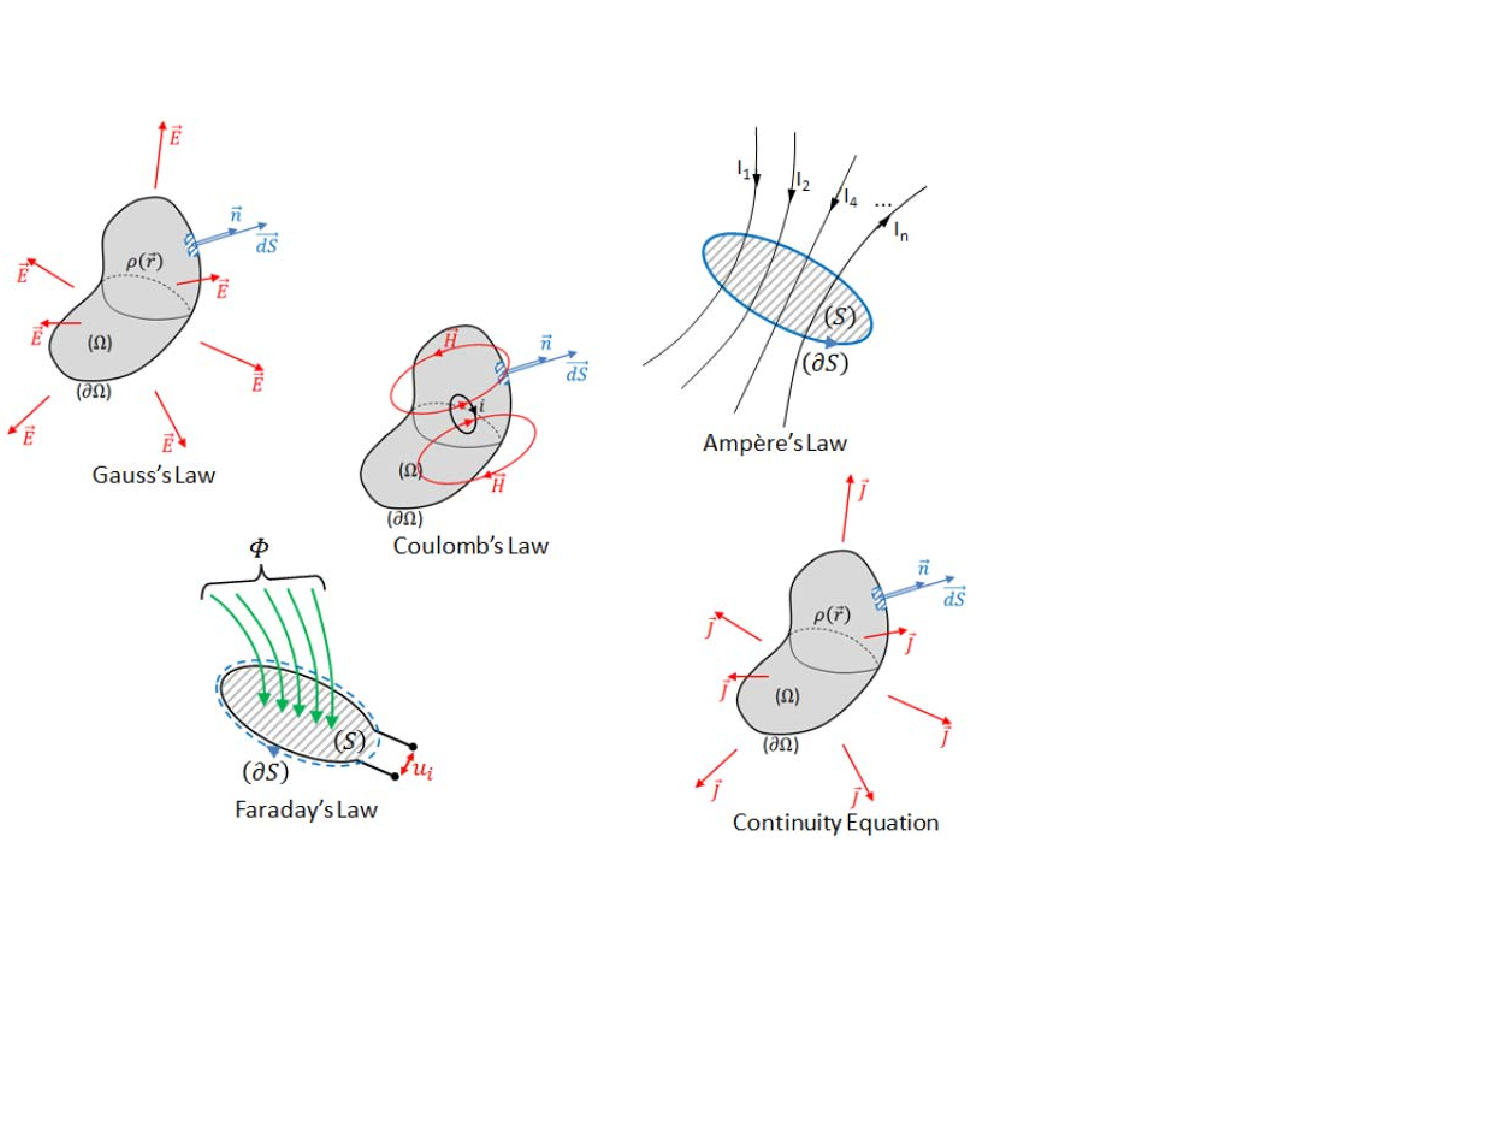
\includegraphics[width=.55\textwidth]{./images/MaxwellEqImages.pdf}
\end{figure}

\subsection{Maxwell Equations in time domain}
Using Gauss Theorem on Equation (\ref{eq:MaxwellInt1}) and (\ref{eq:MaxwellInt2}) and Stokes Theorem on (\ref{eq:MaxwellInt3}) and (\ref{eq:MaxwellInt4}) the following Maxwell Equations in time domain can be obtained as 
\begin{multicols}{2}
	\begin{equation}
		\nabla \cdot \vec{D} = \rho
		\label{eq:MaxwellDiff1_1}
	\end{equation}
	\begin{equation}
		\nabla \cdot \vec{B} = 0
		\label{eq:MaxwellDiff1_2}
	\end{equation}
	\begin{equation}
		\nabla \times \vec{H} = \vec{J} + \frac{\partial \vec{D}}{\partial t} = \sigma \vec{E} + \varepsilon \frac{\partial \vec{E}}{\partial t}
		\label{eq:MaxwellDiff1_3}
	\end{equation}
	\begin{equation}
		\nabla \times \vec{E} = - \frac{\partial \vec{B}}{\partial t}
		\label{eq:MaxwellDiff1_4}
	\end{equation}
	
	\begin{equation}
		\nabla \cdot \vec{E} = \frac{\rho}{\varepsilon}
		\label{eq:MaxwellDiff2_1}
	\end{equation}
	\begin{equation}
		\nabla \cdot \vec{H} = 0
		\label{eq:MaxwellDiff2_2}
	\end{equation}
	\begin{equation}
		\nabla \times \vec{B} = \mu\left(\vec{J} + \frac{\partial \vec{D}}{\partial t}\right)
		\label{eq:MaxwellDiff2_3}
	\end{equation}
	\begin{equation}
		\nabla \times \vec{E} = -\mu \frac{\partial \vec{H}}{\partial t}
		\label{eq:MaxwellDiff2_4}
	\end{equation}
\end{multicols}
where Equation (\ref{eq:MaxwellDiff1_3}) and (\ref{eq:MaxwellDiff2_3}) show $\vec{H} \rightarrow \vec{E}$ coupling and Equation (\ref{eq:MaxwellDiff1_4}) and (\ref{eq:MaxwellDiff2_4}) show $\vec{E} \rightarrow \vec{H}$ coupling.

\subsection{Maxwell Equations in frequency domain}
If the field sources are harmonic sinusoidal time functions, the fields must have also this time dependence if the involved materials are linear. The fields can be represented as the following complex vectors
\begin{equation*}
	\vec{F}\left(\vec{r},t\right) = \Re\{\underline{\vec{F}}\left(\vec{r}\right) \cdot e^{j\omega t}\}.
\end{equation*}
The main advantage of this approach is the following elimination of the time derivatives
\begin{equation*}
	\frac{\partial}{\partial t}\left(e{j \omega t}\right) = j \omega^\cdot e^{j \omega t}
\end{equation*}
applied to the Maxwell Equations in time domain the following is obtained
\begin{equation*}
	\nabla \cdot \underline{\vec{D}}\left(\vec{r}\right) = \underline{\rho}\left(\vec{r}\right)
\end{equation*}
\begin{equation*}
	\nabla \cdot \underline{\vec{B}}\left(\vec{r}\right) = 0
\end{equation*}
\begin{equation*}
	\nabla \times \underline{\vec{H}}\left(\vec{r}\right) = \underline{\vec{J}}\left(\vec{r}\right) + j \omega \cdot \underline{\vec{D}}\left(\vec{r}\right)
\end{equation*}
\begin{equation*}
	\nabla \times \underline{\vec{E}}\left(\vec{r}\right) = - j\omega \underline{\vec{B}}\left(\vec{r}\right)
\end{equation*}